% ========================================================================
\section*{Installation}
\href{https://auto.gluon.ai/stable/index.html}{AutoGluon} (\href{https://github.com/autogluon/autogluon/}{GitHub}) supports Python 3.9 to 3.12 and is available for Linux, MacOS, and Windows. The fastest way to install AutoGluon is through the \href{https://docs.astral.sh/uv/}{uv package manager}.

\begin{minted}[fontsize=\footnotesize, bgcolor=codeback, frame=leftline, framesep=10pt]{bash}
# Install UV package installer (faster than pip)
pip install -U uv
# Install AutoGluon
python -m uv pip install autogluon
\end{minted}

% ========================================================================

\section*{Preparing Data}

AutoGluon can generate forecasts for datasets consisting of \textbf{multiple univariate} time series. Here we use the \href{https://www.sciencedirect.com/science/article/pii/S0169207019301128}{M4 Competition} Daily dataset to demonstrate how to do forecasting with AutoGluon.

\begin{minted}[fontsize=\footnotesize, bgcolor=codeback, frame=leftline, framesep=10pt]{python}
import pandas as pd
raw_data = pd.read_csv("m4_daily.csv")
raw_data.head()
\end{minted}

\begin{center}
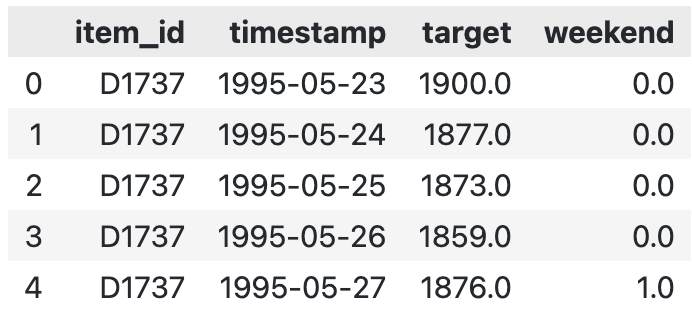
\includegraphics[width=0.6\linewidth]{timeseries/images/raw_data.png}
\end{center}

\medskip

Each row contains unique ID of each time series, timestamp, value of the time series, and (optional) time-varying \textbf{covariates}.

\medskip

A time series datasets may also optionally include time-independent \textbf{static features} (metadata) for each time series.

\begin{minted}[fontsize=\footnotesize, bgcolor=codeback, frame=leftline, framesep=10pt]{python}
static_features = pd.read_csv("m4_metadata.csv")
static_features.head()
\end{minted}

\begin{center}
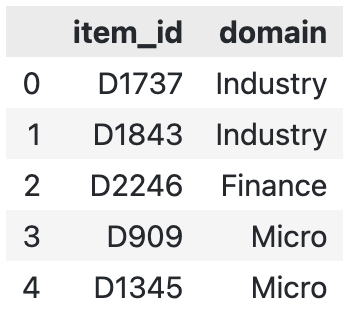
\includegraphics[width=0.30\linewidth]{timeseries/images/static_features.png}
\end{center}

\medskip

We convert raw data into a \textbf{TimeSeriesDataFrame} used by AutoGluon.

\begin{minted}[fontsize=\footnotesize, bgcolor=codeback, frame=leftline, framesep=10pt]{python}
from autogluon.timeseries import TimeSeriesDataFrame
train_data = TimeSeriesDataFrame.from_data_frame(
    raw_data,
    id_column="item_id",
    timestamp_column="timestamp",
    static_features_df=static_features,  # optional
)
\end{minted}


\vfill\null
\columnbreak
% ========================================================================

\section*{Training}

Train models to forecast the values in the column ‘target’ 30 steps into the future for each time series.

\begin{minted}[fontsize=\footnotesize, bgcolor=codeback, frame=leftline, framesep=10pt]{python}
from autogluon.timeseries import TimeSeriesPredictor
predictor = TimeSeriesPredictor(
    target="target",
    prediction_length=30,
).fit(train_data, presets="medium_quality")
\end{minted}

More options to construct a \textbf{TimeSeriesPredictor} instance (\href{https://auto.gluon.ai/stable/api/autogluon.timeseries.TimeSeriesPredictor.html}{docs}):

\begin{minted}[fontsize=\footnotesize, bgcolor=codeback, frame=leftline, framesep=10pt]{python}
# The metric used to tune models
eval_metric="MASE"
# Select quantiles for the probabilistic forecast
quantile_levels = [0.1, 0.5, 0.9]
# If data has irregular timestamps, provide frequency
freq="D"
# Covariates that are known in the future
# (e.g., holidays, promotions, weather forecasts)
known_covariates_names=["weekend"]
\end{minted}
More options for the \textbf{fit} method (\href{https://auto.gluon.ai/stable/api/autogluon.timeseries.TimeSeriesPredictor.fit.html}{docs}):

\begin{minted}[fontsize=\footnotesize, bgcolor=codeback, frame=leftline, framesep=10pt]{python}
# Limit the training time, in seconds
time_limit=600
# More accurate forecasts but longer training time
presets="best_quality"
# Backtest using multiple validation windows
num_val_windows=3
# Manually select what models to use,
# e.g., only use ETS and Chronos-Bolt (Base)
hyperparameters={
    "ETS": {"seasonal_period": 14},
    "Chronos": {"model_path": "bolt_base"},
}
# Ignore some models
excluded_model_types=["AutoARIMA", "PatchTST"]
\end{minted}



\section*{Monitoring}
Understand the contribution of each model.

\begin{minted}[fontsize=\footnotesize, bgcolor=codeback, frame=leftline, framesep=10pt]{python}
predictor.leaderboard()
\end{minted}

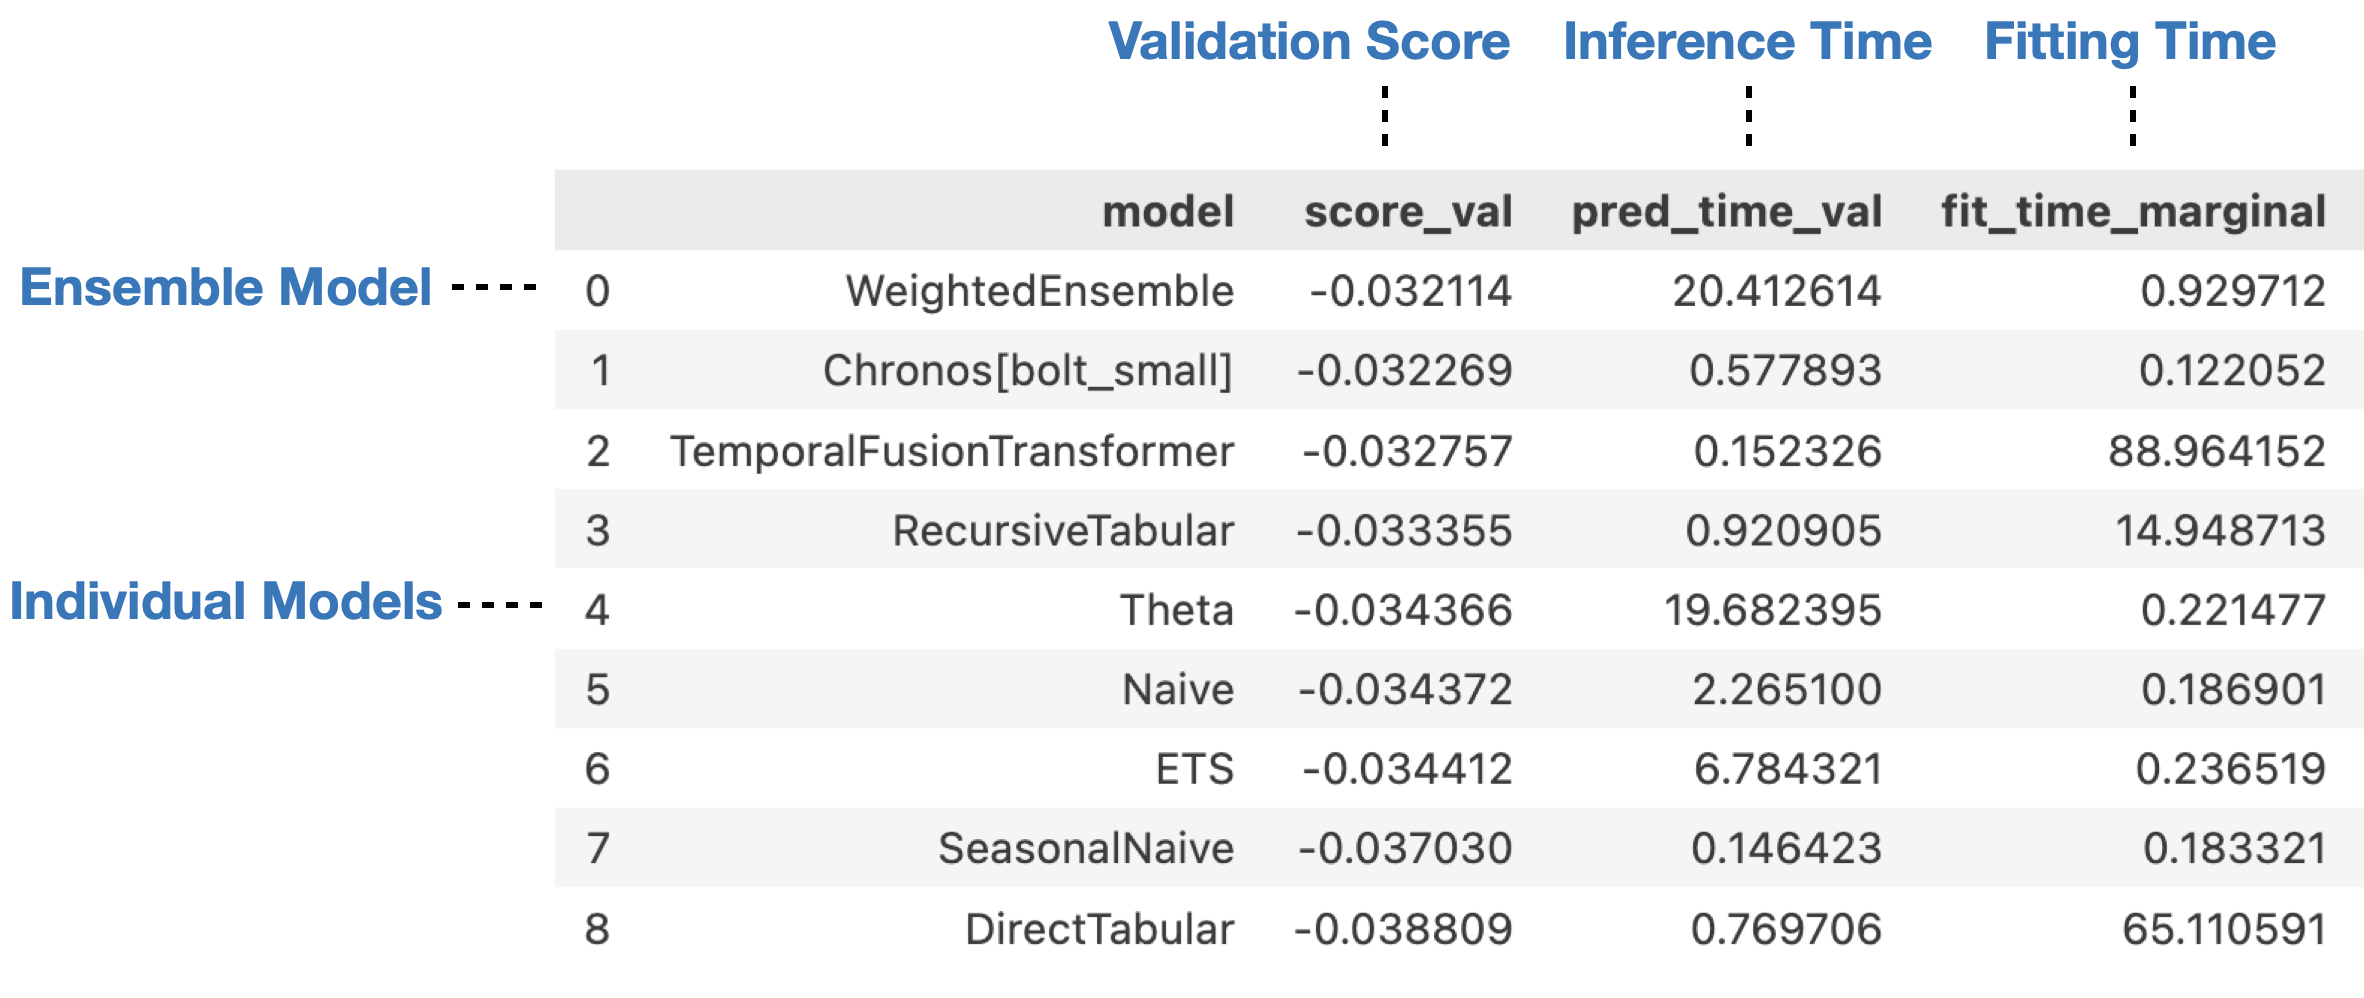
\includegraphics[width=\linewidth]{timeseries/images/leaderboardv1.2-medium_quality.png}

\vfill\null
\columnbreak
% ========================================================================

\section*{Predicting}
Forecast \texttt{prediction\_length} steps into the future starting from the end of each time series in \texttt{train\_data}.
\begin{minted}[fontsize=\footnotesize, bgcolor=codeback, frame=leftline, framesep=10pt]{python}
predictions = predictor.predict(
    train_data,
    # only necessary if known_covariates_names
    # were provided when creating predictor
    known_covariates=known_covariates,
)
known_covariates.head()
\end{minted}
\vspace{-5mm}
\begin{center}
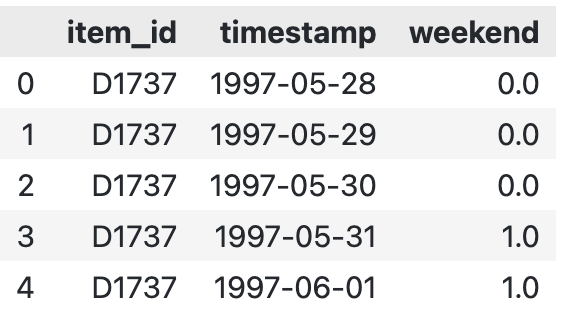
\includegraphics[width=0.35\linewidth]{timeseries/images/future_known_covariates.png}
\end{center}

\medskip

AutoGluon generated probabilistic forecasts that include
\begin{itemize}
    \item mean forecast --- expected value of the time series
    \item quantile forecast --- range of possible outcomes
\end{itemize}

\begin{center}
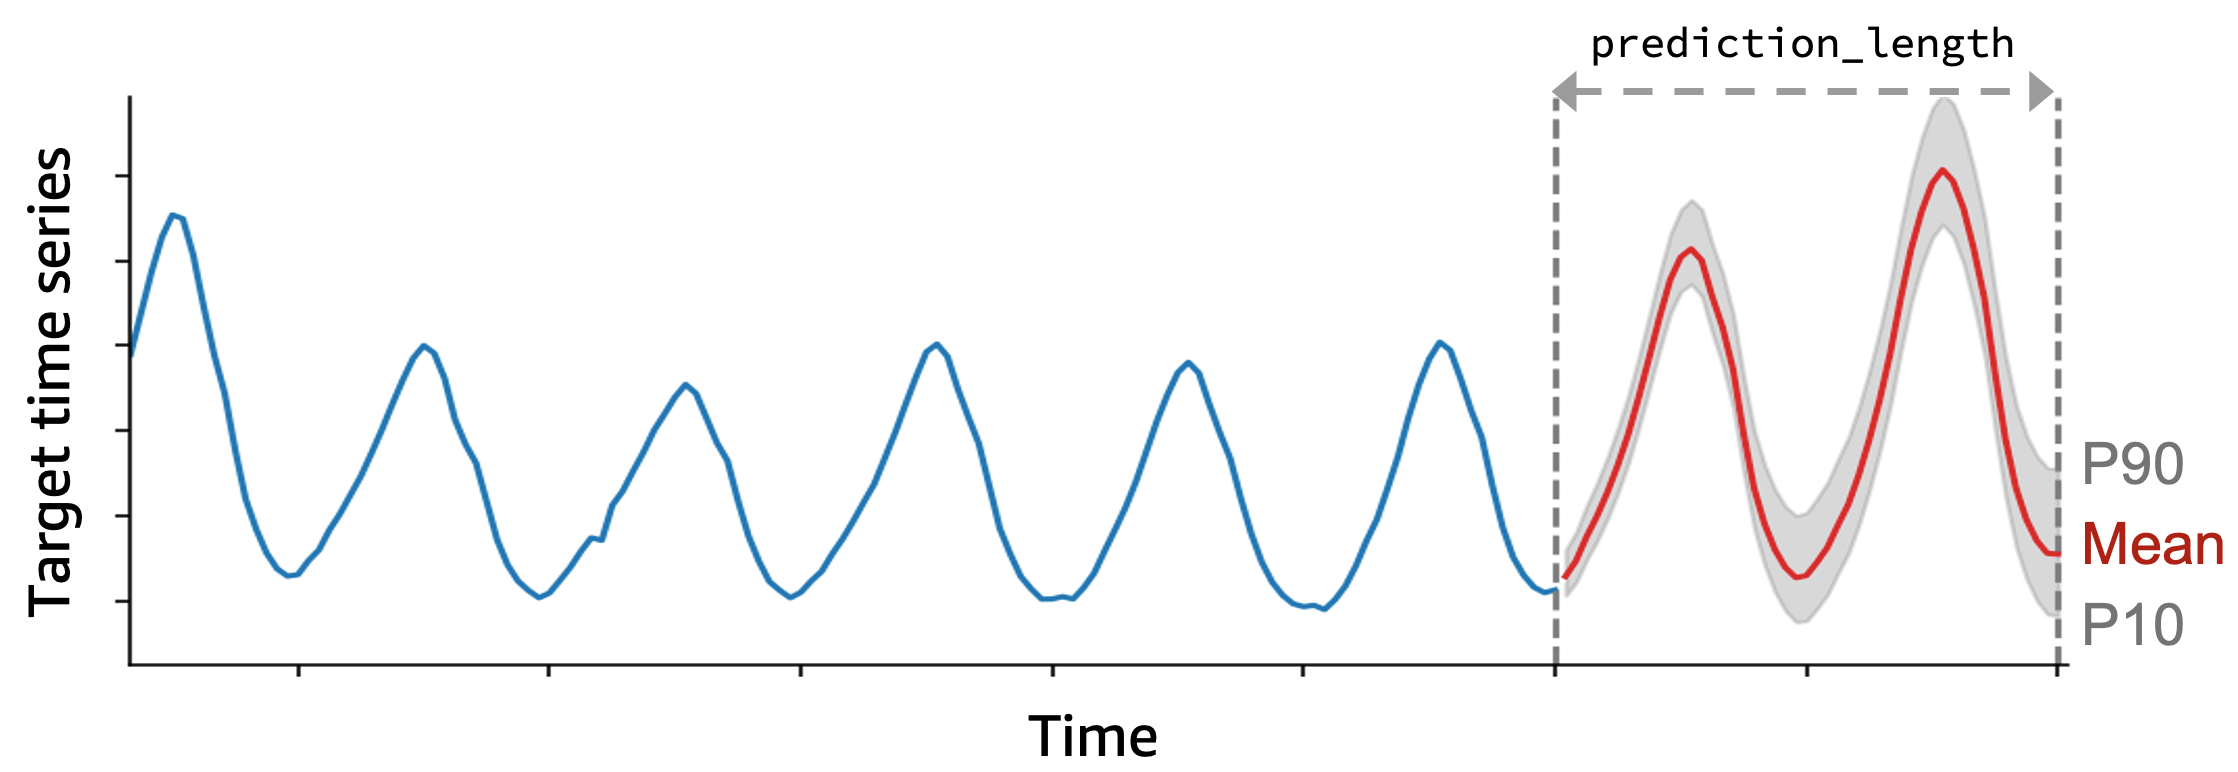
\includegraphics[width=0.95\linewidth]{timeseries/images/probabilistic_forecast.png}
\end{center}

\begin{minted}[fontsize=\footnotesize, bgcolor=codeback, frame=leftline, framesep=10pt]{python}
predictions.head()
\end{minted}

\begin{center}
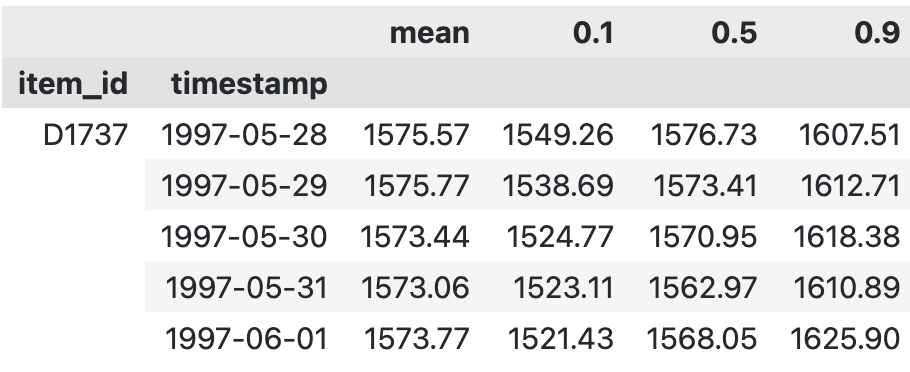
\includegraphics[width=0.6\linewidth]{timeseries/images/predictions.png}
\end{center}

\medskip

AutoGluon predicts with the final ensemble model. You can also predict using an individual model. 

\begin{minted}[fontsize=\footnotesize, bgcolor=codeback, frame=leftline, framesep=10pt]{python}
models = predictor.model_names()
predictor.predict(test_data, model=models[1])
\end{minted}




\begin{itemize}
  \item \href{https://auto.gluon.ai/stable/tutorials/timeseries/index.html}{Detailed  time series tutorials}.
  \item For other types of data, check
  \href{https://auto.gluon.ai/stable/tutorials/tabular/index.html}{TabularPredictor} for tabular data and 
  \href{https://auto.gluon.ai/stable/tutorials/multimodal/index.html}{MultiModalPredictor} for multi-modal data such as images and text. 
  \item Check the \href{https://auto.gluon.ai/stable/cheatsheet.html}{latest version of this cheat sheet}.
  \item Any questions? \href{https://github.com/autogluon/autogluon/discussions}{Ask here}
  \item Like what you see? Consider \href{https://github.com/autogluon/autogluon/stargazers}{starring AutoGluon on GitHub} and \href{https://twitter.com/autogluon}{following us on X (Twitter)} to get notified of the latest updates!
\end{itemize}

% ========================================================================

\raggedcolumns


% \begin{minted}[fontsize=\footnotesize, bgcolor=codeback, frame=leftline, framesep=10pt]{python}
% \end{minted}
